% ------------------------------------------------------------------------------
% TYPO3 Version 10 LTS - What's New (English Version)
%
% @author	Michael Schams <schams.net>
% @license	Creative Commons BY-NC-SA 3.0
% @link		https://typo3.org/help/documentation/whats-new/
% @language	English
% ------------------------------------------------------------------------------

\section{Form Framework}
\begin{frame}[fragile]
	\frametitle{Form Framework}

	\begin{center}\huge{\color{typo3darkgrey}\textbf{Form Framework}}\end{center}
	\begin{center}\large{\textit{Creating and managing forms made easier}}\end{center}

\end{frame}

% ------------------------------------------------------------------------------
% Feature | 79445 | Add Multistep Wizard

\begin{frame}[fragile]
	\frametitle{Form Framework}
	\framesubtitle{Multi-step Wizard}

	\begin{itemize}
		\item A new JavaScript module \texttt{MultiStepWizard} has been introduced,
			that adds the following features:

			\begin{itemize}
				\item Navigation to previous steps.
				\item Steps support descriptive labels such as "Start" or "Finish", rather than the numerical indicator "Step x of y".
				\item Optimized configuration structure.
			\end{itemize}

		\item See \href{https://docs.typo3.org/c/typo3/cms-core/master/en-us/Changelog/10.2/Feature-79445-AddMultistepWizard.html}{change log}
			for JavaScript code examples.

		\item This new features improves the user experience significantly: backend users will notice an enhanced form creation wizard.

	\end{itemize}

\end{frame}

% ------------------------------------------------------------------------------
% Feature | 84757 | Double click in structure tree changes label

\begin{frame}[fragile]
	\frametitle{Backend User Interface}
	\framesubtitle{Edit Titles}

	Labels of form elements can now be edited by double clicking on the title in the structure tree.

	\begin{figure}
		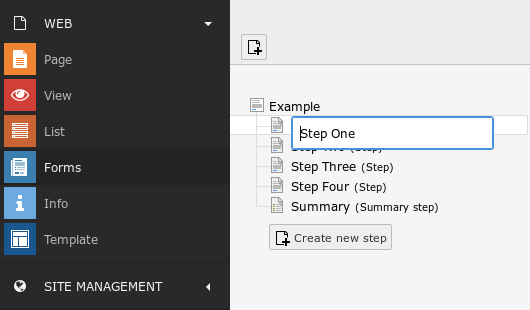
\includegraphics[width=0.5\linewidth]{FormFramework/84757-DoubleClickToChangeLabel.png}
	\end{figure}

\end{frame}

% ------------------------------------------------------------------------------
% Important | 84221 | Restructuring of form setup

\begin{frame}[fragile]
	\frametitle{Form Framework}
	\framesubtitle{Form Setup}

	\begin{itemize}
		\item Three files were used previously: \texttt{BaseSetup.yaml}, \texttt{FormEditorSetup.yaml}, and \texttt{FormEngineSetup.yaml}.
		\item This has been streamlined and consolidated into one file now: \texttt{FormSetup.yaml}.
		\item This file contains the basic setup including imports of the configuration for validators, form elements and finishers.
		\item All previously used inheritances and mixins have been resolved which makes it very easy to understand the entire configuration.
	\end{itemize}

\end{frame}

% ------------------------------------------------------------------------------
% Breaking | 87009 | Use multiple translation files by default in EXT:form

\begin{frame}[fragile]
	\frametitle{Form Framework}
	\framesubtitle{Translations}

	% decrease font size for code listing
	\lstset{basicstyle=\tiny\ttfamily}

	\begin{itemize}
		\item The following option has been renamed:\newline
			\small\texttt{translationFile} \textrightarrow\hspace{0.1cm}\texttt{translationFiles}\normalsize
		\item The default translation files are now registered at index 10:

			\begin{itemize}
				\item \texttt{EXT:form/Resources/Private/Language/locallang.xlf}
				\item \texttt{EXT:form/Resources/Private/Language/Database.xlf}
			\end{itemize}

		\item Custom form YAML configuration files need to be updated.
\begin{lstlisting}
OLD:
translationFile: path/to/locallang.xlf

NEW:
translationFiles:
  20: path/to/locallang.xlf
\end{lstlisting}

	\end{itemize}

\end{frame}

% ------------------------------------------------------------------------------
% Feature | 84203 | Unify form setup YAML loading

\begin{frame}[fragile]
	\frametitle{Form Framework}
	\framesubtitle{YAML Files}

	\begin{itemize}
		\item YAML files now use the TYPO3 core YAML file loader.
		\item This enabled features such as:

			\begin{itemize}
				\item Import of other YAML files via \texttt{imports} directive.
				\item Replacement of \texttt{\%placeholders\%}.
			\end{itemize}

	\end{itemize}

\end{frame}

% ------------------------------------------------------------------------------
% Feature | 90052 | Form YAML configuration available in configuration module

\begin{frame}[fragile]
	\frametitle{Form Framework}
	\framesubtitle{YAML Configuration}

	\begin{columns}[T]
		\begin{column}{.04\textwidth}
		\end{column}
		\begin{column}{.38\textwidth}

			If the system extension \texttt{EXT:form} is installed, the parsed YAML configuration
			can be displayed under \textbf{SYSTEM} $\rightarrow$ \textbf{Configuration}.

			\vspace{0.2cm}

			This also requires administrators to activate \texttt{EXT:lowlevel} of course.

		\end{column}
		\begin{column}{.58\textwidth}
			\vspace{-0.3cm}
			\begin{figure}
				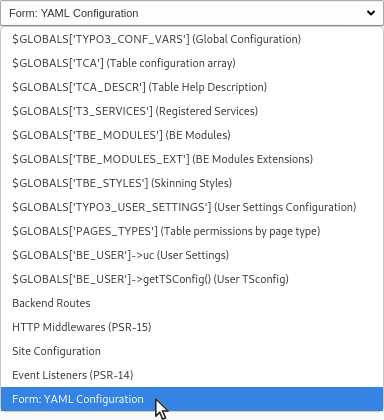
\includegraphics[width=0.70\linewidth]{FormFramework/90052-AddYamlConfigurationToConfigurationModule.png}
			\end{figure}
		\end{column}
	\end{columns}

\end{frame}

% ------------------------------------------------------------------------------
% Feature | 89747 | Custom tables with record browser in forms

\begin{frame}[fragile]
	\frametitle{Form Framework}
	\framesubtitle{Record Browser}

	% decrease font size for code listing
	\lstset{basicstyle=\tiny\ttfamily}

	\begin{itemize}
		\item The record browser can now be configured to use custom tables:
\begin{lstlisting}
TYPO3:
  CMS:
    Form:
      prototypes:
        standard:
          formElementsDefinition:
            MyCustomElement:
              formEditor:
                editors:
                  # ...
                  300:
                    identifier: myRecord
                    # ...
                    browsableType: tx_myext_mytable
                    propertyPath: properties.myRecordUid
                    # ...
\end{lstlisting}

	\end{itemize}

\end{frame}

% ------------------------------------------------------------------------------
% Feature | 89746 | Custom icon for record browser button in forms

\begin{frame}[fragile]
	\frametitle{Form Framework}
	\framesubtitle{Record Browser}

	% decrease font size for code listing
	\lstset{basicstyle=\tiny\ttfamily}

	\begin{itemize}
		\item The button icon of the record browser are now configurable:
\begin{lstlisting}
TYPO3:
  CMS:
    Form:
      prototypes:
        standard:
          formElementsDefinition:
            MyCustomElement:
              formEditor:
                editors:
                  # ...
                  300:
                    identifier: contentElement
                    # ...
                    browsableType: tt_content
                    iconIdentifier: mimetypes-x-content-text
                    propertyPath: properties.contentElementUid
                    # ...
\end{lstlisting}

	\end{itemize}

\end{frame}

% ------------------------------------------------------------------------------
% Feature | 84713 | Access single values in form templates

\begin{frame}[fragile]
	\frametitle{Form Framework}
	\framesubtitle{Record Browser}

	% decrease font size for code listing
	\lstset{basicstyle=\tiny\ttfamily}

	\begin{itemize}
		\item A new \textit{RenderFormValue-ViewHelper} lets integrators/developers access single form values in templates:
\begin{lstlisting}
<p>
  The following message was just sent by
  <formvh:renderFormValue renderable="{page.rootForm.elements.name}" as="formValue">
    {formValue.processedValue}
  </formvh:renderFormValue>:
</p>

<blockquote>
  <formvh:renderFormValue renderable="{page.rootForm.elements.message}" as="formValue">
    {formValue.processedValue}
  </formvh:renderFormValue>
</blockquote>
\end{lstlisting}

	\end{itemize}

\end{frame}

% ------------------------------------------------------------------------------
% Feature | 82706 | Render fieldset labels in form templates

\begin{frame}[fragile]
	\frametitle{Form Framework}
	\framesubtitle{Fieldset Labels}

	\begin{itemize}
		\item The section element \texttt{Fieldset} is now accessible in templates.
		\item By default this affects the \textbf{SummaryPage} form element as well as the \textbf{EmailToReceiver} and \textbf{EmailToSender} finishers.
		\item Typical use-case:\newline
			\small
				A form with a shipping and a billing address. Both sections could have a field with the same name, e.g. \texttt{street}.
				It is now possible to distinguish between both fields by using fieldset labels.
			\normalsize

	\end{itemize}

\end{frame}

% ------------------------------------------------------------------------------
% Deprecation | 88238 | Allowed MIME types of FileUpload and ImageUpload

\begin{frame}[fragile]
	\frametitle{Form Framework}
	\framesubtitle{File Uploads}

	\begin{itemize}
		\item Predefined \texttt{allowedMimeTypes} of the following form elements have been marked \textbf{deprecated}:

			\begin{itemize}
				\item \texttt{FileUpload}
				\item \texttt{ImageUpload}
			\end{itemize}

		\item All valid MIME types must be explicitly listed in the form definition now\newline
			\smaller
				(predefined MIME types will be removed in TYPO3 v11)
			\normalsize

	\end{itemize}

\end{frame}

% ------------------------------------------------------------------------------
% Deprecation | 89742 | Form mixins

\begin{frame}[fragile]
	\frametitle{Form Framework}
	\framesubtitle{Form Mixins}

	\begin{itemize}
		\item Mixins have been marked as \textbf{deprecated} and should not be used anymore.
		\item This affects all inheritances from \texttt{TYPO3.CMS.Form.mixins.*}.
		\item Migration options:

			\begin{itemize}
				\item Embed the essential parts from \texttt{TYPO3.CMS.Form.mixins.*}, or
				\item migrate them to custom mixins.
			\end{itemize}

	\end{itemize}

\end{frame}

% ------------------------------------------------------------------------------
% Feature | 80420 | Allow multiple recipients in email finisher

\begin{frame}[fragile]
	\frametitle{Form Framework}
	\framesubtitle{Multiple Recipients}

	\begin{itemize}
		\item Mails sent by the \textit{EmailFinisher} can now have multiple recipients.

		\item The following new options have been introduced:

			\begin{itemize}
				\item \texttt{recipients} (To)
				\item \texttt{replyToRecipients} (Reply-To)
				\item \texttt{carbonCopyRecipients} (CC)
				\item \texttt{blindCarbonCopyRecipients} (BCC)
			\end{itemize}

	\end{itemize}

\end{frame}

% ------------------------------------------------------------------------------
% Feature | 80420 | Allow multiple recipients in email finisher

\begin{frame}[fragile]
\frametitle{Form Framework}
\framesubtitle{Multiple Recipients}

	% decrease font size for code listing
	\lstset{basicstyle=\tiny\ttfamily}

	\begin{itemize}
		\item This change requires a manual migration of single value options to their list value successors.

		\smaller\textbf{Old} Finisher configuration:\normalsize
\begin{lstlisting}
finishers:
  -
    identifier: EmailToReceiver
    options:
      recipientAddress: user@example.com
      recipientName: 'Firstname Lastname'
\end{lstlisting}

		\smaller\textbf{New} Finisher configuration:\normalsize
\begin{lstlisting}
finishers:
  -
    identifier: EmailToReceiver
    options:
      recipients:
        user@example.com: 'Firstname Lastname'
\end{lstlisting}

		\item See \href{https://docs.typo3.org/c/typo3/cms-core/10.0/en-us/Changelog/master/Deprecation-80420-EmailFinisherSingleAddressOptions.html}{change log}
			for more migration examples.

	\end{itemize}

\end{frame}

% ------------------------------------------------------------------------------
% Deprecation | 87200 | EmailFinisher format option
% Deprecation | 87200 | EmailFinisher FORMAT_* constants

\begin{frame}[fragile]
	\frametitle{Form Framework}
	\framesubtitle{Plaintext/HTML}

	\begin{itemize}
		\item Mails sent by the \textit{EmailFinisher} can now feature both plaintext and/or HTML part.

		\item At the same time the option \texttt{format} has been marked deprecated and will be removed in TYPO3 v11.

		\item Existing values will be automatically migrated:

			\begin{itemize}\smaller
				\item \texttt{format:html} \tabto{3cm}\textrightarrow\hspace{0.1cm}\texttt{addHtmlPart:\textbf{true}}
				\item \texttt{format:plaintext} \tabto{3cm}\textrightarrow\hspace{0.1cm}\texttt{addHtmlPart:\textbf{false}}
				\item a missing "\texttt{format}" \tabto{3cm}\textrightarrow\hspace{0.1cm}\texttt{addHtmlPart:\textbf{true}}
			\end{itemize}\normalsize

		\item Developers should be aware of the following two constants which have been marked deprecated:

			\begin{itemize}\smaller
				\item \texttt{EmailFinisher::FORMAT\_PLAINTEXT}
				\item \texttt{EmailFinisher::FORMAT\_HTML}
			\end{itemize}\normalsize

	\end{itemize}

\end{frame}

% ------------------------------------------------------------------------------
% Feature | 87798 | Provide a way to sort form lists in ext:form

\begin{frame}[fragile]
	\frametitle{In-depth Changes}
	\framesubtitle{Sorting of Forms}

	% decrease font size for code listing
	\lstset{basicstyle=\tiny\ttfamily}

	\begin{itemize}
		\item Forms can now be sorted in either ascending or descending order.
		\item Two new settings were introduced: \texttt{sortByKeys} and \texttt{sortAscending}.
		\item Forms are initially sorted by their name and their file UID (ascending).
		\item To change the sorting, the following configuration needs to be added in the YAML configuration file:
\begin{lstlisting}
TYPO3:
  CMS:
    Form:
      persistenceManager:
        sortByKeys: ['name', 'fileUid']
        sortAscending: true
\end{lstlisting}

	\end{itemize}

\end{frame}

% ------------------------------------------------------------------------------
